\chapter{Validation}

In the following chapter we'll discuss the results of the formerly
presented implementation, highlighting the benchmarks of the solutions proposed.
In the first part of the chapter we'll investigate the performance of the machine learning
library, in the various situation that may happen. In the following part we will
test the advantages of our microservice oriented architecture with the classical approach
for integration.

\section{Validating Speaker Recognition}

This section is dedicated to the various tests to investigate
the effectiveness in a home security scenario. For our
tests we used two different libraries, comparing their results:
\textit{voiceid} for speaker diarization and identification, \textit{recognito}
for speaker identification only. Furthermore we have used standard configurations
for all the audio files: .wav format, with a frequency 48 kHz and using 16 bit for sampling.

\subsection{Testing the basic model}

Before starting with more complex test it is mandatory to see the effectiveness
of the models in the optimal situation. For the optimal situation we'll take
a unique recording dividing it in the typical machine learning split: 80\% learning
and 20\% for testing the model.\newline
The first test will focus on a batch of voices taken from different sources:

\begin{itemize}
    \item Youtube -  A youtuber using High Quality input camera, using a model with a duration of 50 seconds.
    \item The integrated microphone in my laptop using a model with a duration of 16 seconds.
    \item Voice recordings from Voxforge using a model with a duration 32 seconds.
\end{itemize}
In this scenario the model audio durations will be of different durations and different
quality, we will make more specific tests later in the document.

\subsubsection{Results}

In the following table we summarize the results from the test, where \textit{score} is the
likelihood percentage: less than 40\% is unlikely or wrong and 100\% is completely sure.
The remaining fields are the average execution time for the different tests and the mean duration
of the test files.
\begin{table}
    \label{tab:basicres}
\centering
\caption{Basic test results}
\begin{tabular}{|c|c|c|c|} \hline
& \textbf{Score \%} & \textbf{Avg Execution (ms)} & \textbf{Avg Duration (s)}\\ \hline
\textbf{Youtuber} & 92.7 & 3217 & 56 \\ \hline
\textbf{Myself} & 81.75 & 2524 & 9.25  \\ \hline
\textbf{Voxforge} & 100 & 2665 & 5.5  \\ \hline
\end{tabular}
\end{table}

As can be seen in \ref{tab:basicres}, the \textit{recognito} library works as expected with
different sources and different quality, proving its correctness for the basic functionalities.
However, we can see a difference in the score of the results depending from the source of the
audio recording. The less quality input, the microphone, has a lower score percentage which is very likely
due to the input quality. It is indeed interesting to notice the perfect score of the audios
taken from \textit{Voxforge}. Although their quality is lower than the Youtube video, their
precision is remarkably high. It is also important to notice the discrepancy between the model
audio durations, which doesn't seem to be affect the score too much. We'll try
to see which is the best duration for a model in the next subsection.

\subsubsection{Finding the optimal length for a Model}

The audio recordings used as model in the former chapter are all of different durations.
However, in order to have a more refined comparison we need to know the best duration of a model
for the best match.\newline
The test will be executed trimming the audio model file in different slots of time, relatively:
1 second, 3 seconds, 5 seconds, 10 seconds and 15 seconds. The models are the same ones
from the previous test.
\pgfplotsset{width=10cm,compat=1.9}

\begin{center}


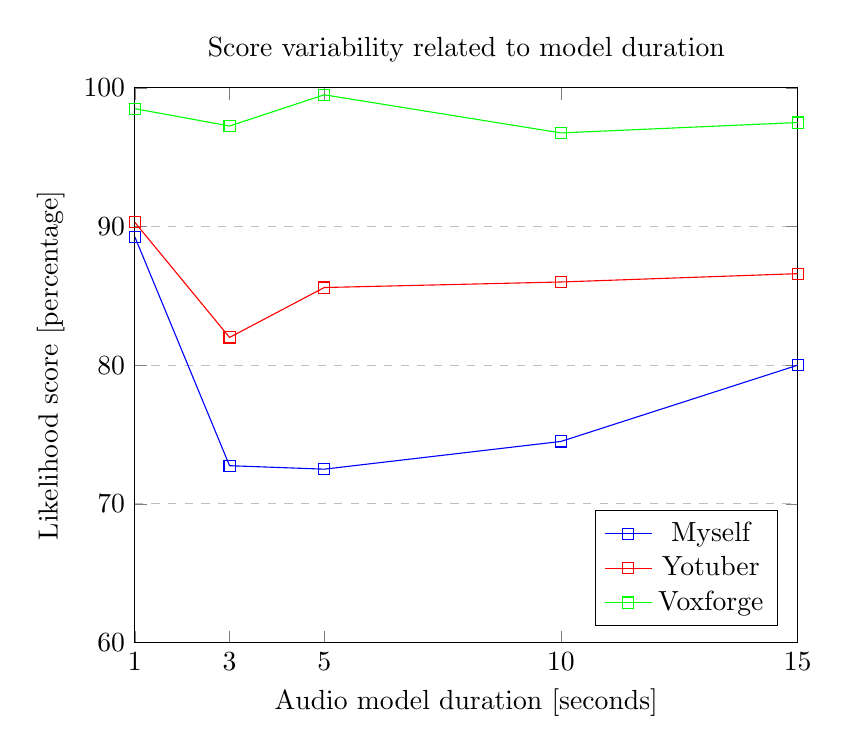
\begin{tikzpicture}

\begin{axis}[
    title={Score variability related to model duration},
    xlabel={Audio model duration [seconds]},
    ylabel={Likelihood score [percentage]},
    xmin=1, xmax=15,
    ymin=60, ymax=100,
    xtick={1,3,5,10,15},
    ytick={60,70,80,90,100},
    legend pos=south east,
    ymajorgrids=true,
    grid style=dashed,
]

\addplot[
    color=blue,
    mark=square,
    ]
    coordinates {
    (1,89.25)(3,72.75)(5,72.5)(10,74.5)(15,80)
    };
\addplot[
    color=red,
    mark=square,
    ]
    coordinates {
    (1,90.3)(3,82)(5,85.6)(10,86)(15,86.6)
    };
\addplot[
    color=green,
    mark=square,
    ]
    coordinates {
    (1,98.5)(3,97.25)(5,99.5)(10,96.75)(15,97.5)
    };
    \legend{Myself,Yotuber,Voxforge}

\end{axis}
\end{tikzpicture}
\end{center}

Surprisingly, as can be seen in the chart above, we had the best results with the
1 second audio model duration. However it is not a good choice to consider this length,
which in some test recordings led to a mismatch in the speaker match. This was more clear
when considering different people from a low quality input (the laptop's microphone),
matching 2 times the wrong person. The mismatch didn't occur with the longer audio models.
It is also interesting to note the fall of the likelihood score for all the models when considering
a slightly longer duration for the audio. This is can be attributed to the noise introduced into the learning process
by some silence in the recording, altering the identification process. The matching
rate starts increasing and slowly normalizing to the optimal matching value approximately
between 10 and 15 seconds.\newline
Despite the fact that this time we used same duration audio models, the test audio segments
were each one of a different duration. In the next section we'll test which is the best duration
for a segment to perform a good match, using the 15 seconds model as the best for our situation.

\subsubsection{Finding the optimal length for an Audio Segment}

As introduced in the previous sections in our scenario we decided to split a single
long audio recording in smaller segments. The question is now to find the optimal duration
for a segment. We will use as model each relative optimal from the previous test, and apply to them
various test model of the following duration length: 1 second, 3 seconds, 5 seconds, 7 seconds,
11 seconds and 13 seconds.

\begin{center}


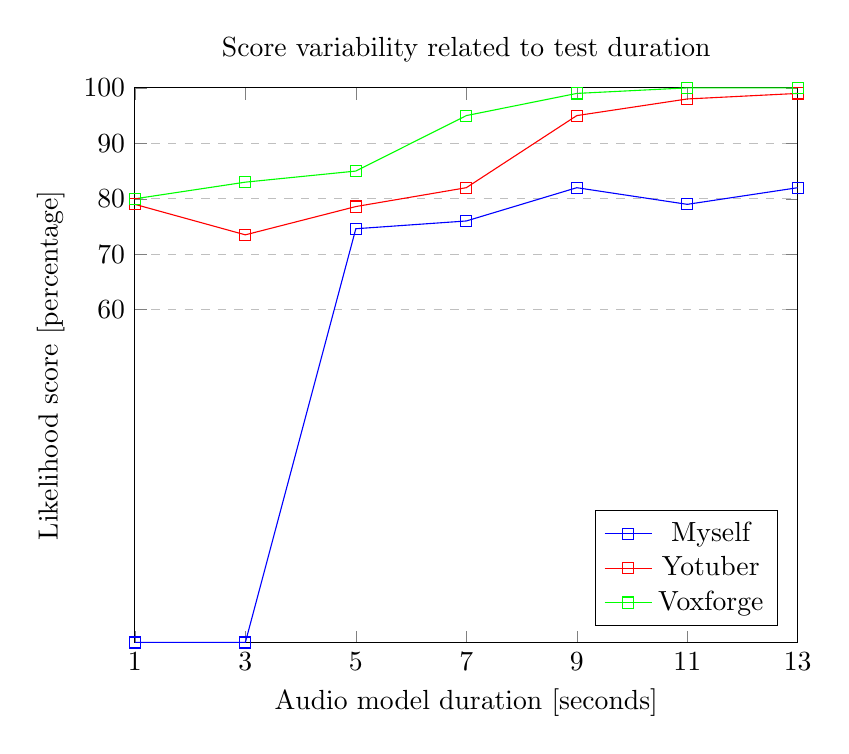
\begin{tikzpicture}

\begin{axis}[
    title={Score variability related to test duration},
    xlabel={Audio model duration [seconds]},
    ylabel={Likelihood score [percentage]},
    xmin=1, xmax=13,
    ymin=0, ymax=100,
    xtick={1,3,5,7,9,11,13},
    ytick={60,70,80,90,100},
    legend pos=south east,
    ymajorgrids=true,
    grid style=dashed,
]

\addplot[
    color=blue,
    mark=square,
    ]
    coordinates {
    (1,0)(3,0)(5,74.6)(7,76)(9,82)(11,79)(13,82)
    };
\addplot[
    color=red,
    mark=square,
    ]
    coordinates {
    (1,79)(3,73.5)(5,78.6)(7,82)(9,95)(11,98)(13,99)
    };
\addplot[
    color=green,
    mark=square,
    ]
    coordinates {
    (1,80)(3,83)(5,85)(7,95)(9,99)(11,100)(13,100)
    };
    \legend{Myself,Yotuber,Voxforge}

\end{axis}
\end{tikzpicture}
\end{center}

As can be seen from the chart, the matching increases linearly with the test duration
length, approaching the best value at 13 seconds.\newline
For short test models the system is unpredictable, though providing generally some
good matches we have noticed some mismatches (marked as 0) for low level inputs. Moreover
these short tests (1 or 3 seconds) seems to be heavily influenced by external noise.\newline
It is also interesting to notice that the running time for the identification process is very slightly
influenced by the length of the duration. This led us to the conclusion that the \textit{13 seconds}
audio duration is the optimal one for our scenario.\newline
Up to now we have used models with different speakers but also from different types of sources. In the
next section we will investigate how the system works when using models applied to the same
speaker but from a different audio source.

\subsection{Testing different inputs with the same speaker}

As seen in the previous tests it is now clear that the input quality influences the output
of the recognition. However we don't know how much the input quality affects the matching,
which we will investigate in the following test. In order to get a qualitative result
we set up the validation using different audio inputs, ranging in quality and with different
devices. In our test we have considered the following devices:

\begin{itemize}
    \item Laptops - usually have a built-in microphone, though the quality
    is not high. Furthermore we used different laptops to see an average likelihood
    score not biased by only one device.
    \item Smartphones - also have an integrated microphone, usually of a higher quality
    since it is one of the key components of a smartphone.
    \item Integrated microphone - many high quality headphones have an integrated
    microphone, typically of better quality then the previous ones.
\end{itemize}

\subsubsection{Results}

\begin{table}
    \label{tab:inputres}
\centering
\caption{Test with different speakers}
\begin{tabular}{|c|c|} \hline
\textbf{Device} & \textbf{Avg Score \%} \\ \hline
\textbf{Laptop} & 83 \\ \hline
\textbf{Smartphone} & 88  \\ \hline
\textbf{Headphones} & 93.6  \\ \hline
\end{tabular}
\end{table}

As can be see in \ref{tab:inputres} there is a definitive difference in the matching score
with different inputs. The test highlighted our assumption, though the error introduced is
not too high. We consider \textgreater 80\% already a good result, though there is only a 10\%
of difference between the lowest quality and the highest in the test. Therefore a halfway
is more then perfect for an accurate recognition.



\subsection{Testing same speaker talking different languages}

One of the many interesting points of speaker recognition is its ability to perform
recognition of people talking different languages. Although it is very unlikely
for people to speak different languages in the same house, it is a characteristic to
validate. In this test we will use different models, all of them based on the reading of a
paragraph in different languages. Therefore we will analyze if there exists any noise or error
in matching introduced by the spoken language into the model. The languages used in the test will be:
English, Italian, German and Spanish. Those languages are chosen based on the speaker's ability to
speak with an accent as appropriate as possible.



\subsubsection{Results}

The results showed only a small variability introduced by the language spoken. Although
the speaker was using different languages the system could recognize the person without
any mismatch and with high likelihood scores. It is interesting to see that the language
which had the lowest match values is English. The reason may be due to the high difference
in the accent with the other languages, whereas Italian and Spanish have a high relative
match score.
\begin{center}


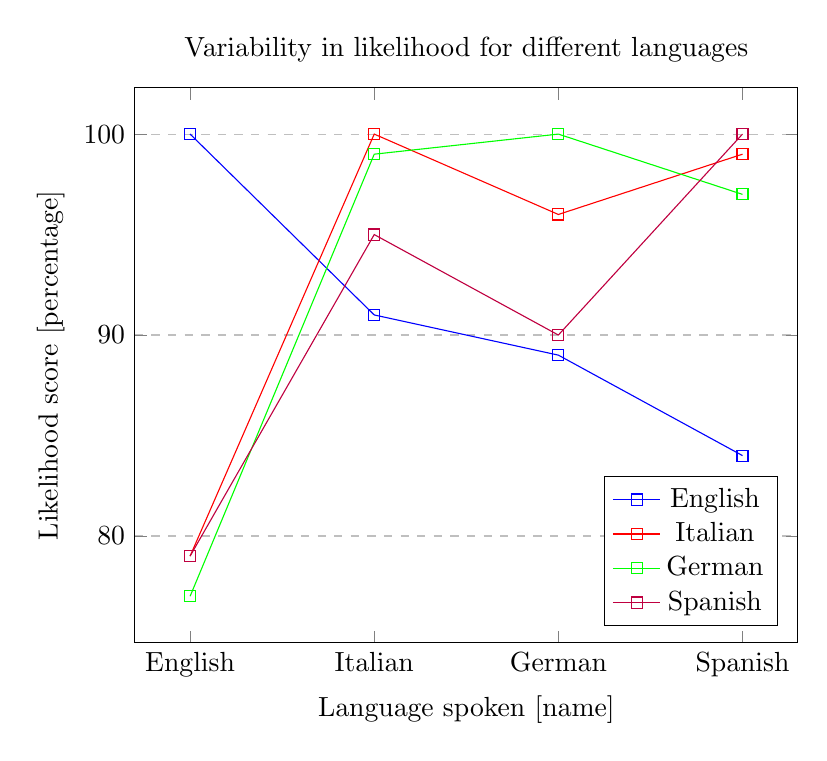
\begin{tikzpicture}

\begin{axis}[
    title={Variability in likelihood for different languages},
    xlabel={Language spoken [name]},
    ylabel={Likelihood score [percentage]},
    symbolic x coords={English,Italian,German,Spanish},
    xtick=data,
    ytick={80,90,100},
    legend pos=south east,
    ymajorgrids=true,
    grid style=dashed,
]

\addplot[
    color=blue,
    mark=square,
    ]
    coordinates {
    (English,100) (Italian,91) (German,89) (Spanish,84)
    };
\addplot[
    color=red,
    mark=square,
    ]
    coordinates {
    (English,79) (Italian,100) (German,96) (Spanish,99)
    };
\addplot[
    color=green,
    mark=square,
    ]
    coordinates {
    (English,77) (Italian,99) (German,100) (Spanish,97)
    };
\addplot[
    color=purple,
    mark=square,
    ]
    coordinates {
    (English,79) (Italian,95) (German,90) (Spanish,100)
    };
    \legend{English,Italian,German,Spanish}

\end{axis}
\end{tikzpicture}
\end{center}



\subsection{Animal Recognition}

Animals, and more specifically pets are one of the typical sources of noise in the house
which may lead to false positives when listening for intruders. The question in this test
is the ability of the system to learn from \textit{"animals"} and recognize them as different identities.
The first test to run is the basic capability of the algorithm to adapt itself to a dog's barking,
and test if it can recognize the dog as familiar. Furthermore the test can be continued by testing
if the model can recognize all dogs apart from human voices. We have used dogs in our examples
only because it is relatively easy to find their barking recorder, though there should be no
difference in using other animal sounds to perform the test (e.g. cats).
Finally it is important to test
the system functionalities when identifying also different kind of animals.

\subsubsection{Animal Identification}

The purpose of this test is to analyze the identification of a dog given a model
and recognize the animal from it. The main purpose is to be able to identify
the dog as animal, and not the dog as a familiar voice. Our assumption is that
given a dog barking sample we will be able to recognize all the dogs and categorize
them as dog instead of human. \newline
However the test results proved us wrong, the system can not recognize dogs from a single
model, at least not precisely. From the test we had a high variance between the results, some
where matching with relatively good scores (around 70\% on average) meanwhile others
were completely failing. Despite the non reliable result, the problem relies in the
difference of dog races, specially on their size. This results in a very different
and wide range of barking sounds hard to summarize in a single model. However, from
the matching examples we inferred the similarity of size and race, which is a hint for
the next test where we will try to verify a dog identity given its bark.

\begin{table}

\centering
\caption{Animal match results}
\label{tab:animalres}
\begin{tabular}{|c|c|} \hline
    \textbf{Matches} & \textbf{Avg Likelihood (\%)} \\ \hline
    6 out of 13 & 74.7 \\ \hline
\end{tabular}
\end{table}

As can be seen in the table above \ref{tab:animalres}, 6 out of 13 matched, with an accuracy of
~46\%, not enough for a general dog recognition but enough to open new leads for different and more
accurate tests.

\subsubsection{Animal Verification}

From the experience of the previous test we can assume that there is an opportunity
for the verification of an animal identity. The purpose of this validation is to
test the ability of the system to recognize a familiar voice, even though it's a dog
barking. This would allow us to decrease the number of false positives due to pet
noise while listening for possible intrusions. \newline
This test will use a single recording of a bark and split it using the optimal
durations for model and test obtained from the previous tests.
This limitation is due to the difficulty of gathering
barks from the same dog in different situations, though the approach should work fine as well.

\subsubsection{Results}

In our simulation we used three different dogs barking of different
sizes and races. As expected from the previous test the system
managed successfully to match the dogs with their relative models. Furthermore,
the accuracy of the match is very high with a minimum of 85\% in the likelihood
for the worst match.

\begin{table}

\centering
\caption{Animal verification}
\label{tab:animalresver}
\begin{tabular}{|c|c|} \hline
    - & \textbf{Avg Likelihood (\%)} \\ \hline
    \textbf{Dog \#1} & 93 \\ \hline
    \textbf{Dog \#2} & 85 \\ \hline
    \textbf{Dog \#3} & 97 \\ \hline
\end{tabular}
\end{table}

As can be seen in table \ref{tab:animalresver}, the results of the different test
show a high likelihood in the match. We can therefore say that speaker recognition
also applies with non human voices, including pets.\newline
Finally we can conclude that a speaker recognition system can be used to reduce the number
of false positives adding the pets in the model.


\subsection{Cheating the Speaker Recognition}

Until now we have demonstrated speaker recognition working, and not, in many different situations.
Another relevant question is if speaker recognition can be affected by fake impersonations,
more accurately mimicking a voice. Voice imitation can be used to bypass security and
surveillance systems, as in our case it would avoid the detection of the intruder.

\subsection{Step Recognition}

In recent years gait recognition gained popularity due to its
non-invasivity and does not require any cooperation from the user.
However, we think it's possible to apply the same thinking to steps,
identifying someone by their steps. It's still a non invasive technique,
and it is supposed to work similarly as it worked for the animal verification.
We will start verifying the base hypothesis: is the steps are actually recognized.
Subsequently we will try the identification with different pairs of shoes and see if
there is any different or the steps matches anyway. Finally we will try to limit the system
using different models of walking, as final verification.

\section{Validation of the Microservice approach}

In this section we will test the differences between the micro-service
oriented approach with the typical integration. The microservice oriented
will surely be a slower approach, mainly due to the impact of the introduced
overhead. However, we will analyze the different approaches in order to establish
the effective impact, evaluating its feasibility in a real world situation.



\subsection{Microservices Oriented integration and Typical integration}

The first and most basic test to run is the running time of the different approaches,
showing the real difference in the execution of the approaches. Profiling the performance
of the two is the easiest way of highlighting the difference.\newline
For this comparison we will run some reading and writing requests for some simulated devices
on the \textit{Nest} ecosystem. The test will dig into the two possible scenarios when interacting with
Nest:Get and Put. More in detail:

\begin{itemize}
    \item GET - will apply on the same device on the same property on both the tests
    \item PUT - will also apply to the same devices and property.
\end{itemize}

\subsubsection{Results}

\begin{table}

\centering
\caption{Animal match results}
\label{tab:nestbasic}
\begin{tabular}{|c|c|c|} \hline
\textbf{Method} &  \textbf{Operation} & \textbf{Avg Execution time (ms)} \\ \hline
    Direct & GET & 0.27 \\ \hline
    Direct & PUT & 0.31 \\ \hline
    Microservice & GET & 4.10 \\ \hline
    Microservice & PUT & 5.76 \\ \hline
\end{tabular}
\end{table}

As expected the running time with the typical integration is smaller. As can be seen
from table \ref{tab:nestbasic} the average running for a \texttt{GET} request with the direct integration is 0.27 ms whereas the average time for
the microservice approach is 4.10 ms. Similar situation for the \texttt{PUT} operation, with an average of 0.31 ms for the first approach and a higher
execution time for the microservices with an average of 5.76 ms.
Therefore the average delay introduced by the microservice chain is,
on average, 4.64 ms, calculated on both of the operations. This is the price to pay for the different approach, a price that is worth the flexibility
given in the structure. Moreover with the advent of faster networks this price given by the inter network communication will drop
significantly, though even now it doesn't invalidate the overall performance.

\begin{center}


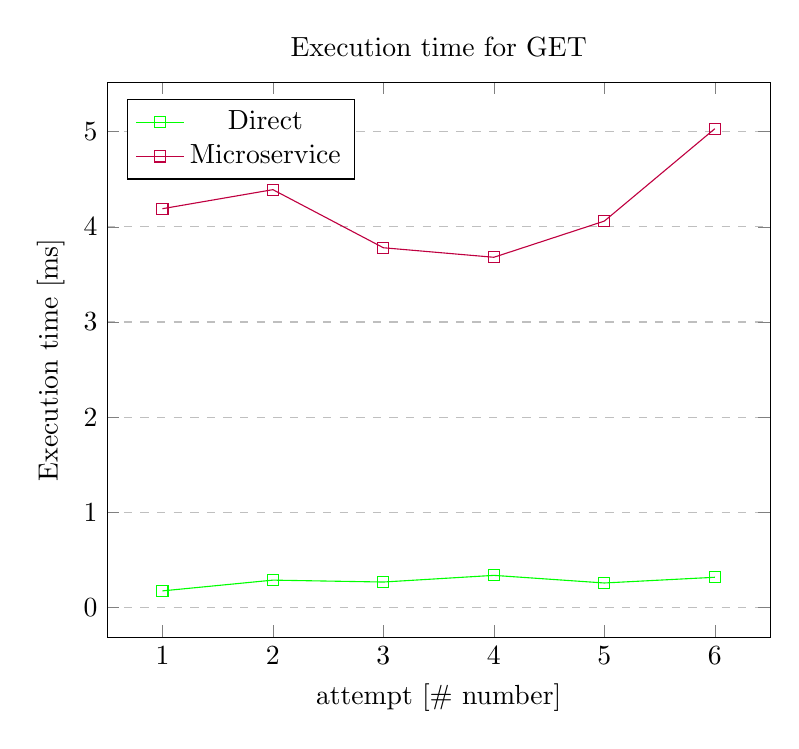
\begin{tikzpicture}

\begin{axis}[
    title={Execution time for GET},
    xlabel={attempt [\# number]},
    ylabel={Execution time [ms]},
    xtick={1,2,3,4,5,6},
    ytick={0,1,2,3,4,5},
    legend pos=north west,
    ymajorgrids=true,
    grid style=dashed,
]
\addplot[
    color=green,
    mark=square,
    ]
    coordinates {
    (1,0.177) (2,0.29) (3,0.27) (4,0.34)  (5,0.26) (6,0.32)
    };
\addplot[
    color=purple,
    mark=square,
    ]
    coordinates {
    (1,4.19) (2,4.39) (3,3.78) (4,3.68) (5,4.06) (6,5.03)
    };
    \legend{Direct,Microservice}

\end{axis}

\end{tikzpicture}

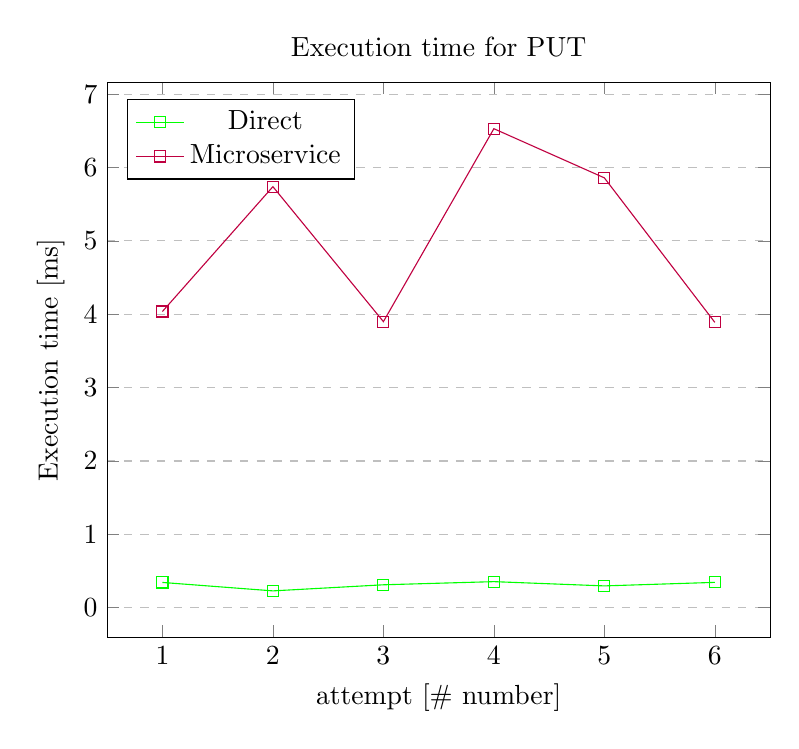
\begin{tikzpicture}

\begin{axis}[
    title={Execution time for PUT},
    xlabel={attempt [\# number]},
    ylabel={Execution time [ms]},
    xtick={1,2,3,4,5,6},
    ytick={0,1,2,3,4,5,6,7},
    legend pos=north west,
    ymajorgrids=true,
    grid style=dashed,
]
\addplot[
    color=green,
    mark=square,
    ]
    coordinates {
    (1,0.344) (2,0.229) (3,0.312) (4,0.355)  (5,0.297) (6,0.345)
    };
\addplot[
    color=purple,
    mark=square,
    ]
    coordinates {
    (1,4.038) (2,5.74) (3,3.9) (4,6.53) (5,5.86) (6,3.89)
    };
    \legend{Direct,Microservice}

\end{axis}

\end{tikzpicture}
\end{center}

\subsection{Architecture limits}

Our architecture, especially in the \textit{HomeKit} situation has some limits
due to the bottleneck given by the web server running on the application. Despite the
fact that all the microservices can scale at need, the service dealing with the homekit
devices has to run as a single instance. In this situation we will try to find the limits
trying to run a high number of requests to the end-point application and see the behavior.\newline
In this scenario we will have many actors (i.e. from 50 to 100), all trying to read or write
a casual property, stressing as much as possible the application.
